\documentclass[12pt]{amsart}
\usepackage{geometry}                % See geometry.pdf to learn the layout options. There are lots.
\geometry{letterpaper, margin=1in}                   % ... or a4paper or a5paper or ... 
%\geometry{landscape}                % Activate for for rotated page geometry
%\usepackage[parfill]{parskip}    % Activate to begin paragraphs with an empty line rather than an indent
\usepackage{graphicx}
\usepackage{amssymb}
\usepackage{epstopdf}
\usepackage{fancyhdr}
\usepackage{wrapfig}
\usepackage[small,bf]{caption}
\setlength{\captionmargin}{0pt}

\DeclareGraphicsRule{.tif}{png}{.png}{`convert #1 `dirname #1`/`basename #1 .tif`.png}

\pagestyle{fancy}
% page 1
\fancypagestyle{first style} {
	\fancyhf{} % clear all existing styles
	\lfoot{\scriptsize %
		Contains Confidential, Proprietary, or Privileged Information \\ %
		Exempt from Public Disclosure \hfill \thepage \hfill Control \#1261-2649%
	}
}
% pages 2 and following
\lhead{\scriptsize %
	DE-FOA-0001261 \\ %
	Concept Paper %
}
\cfoot{} % suppress default center page number
\lfoot{\scriptsize %
	Contains Confidential, Proprietary, or Privileged Information \\ %
	Exempt from Public Disclosure \hfill \thepage \hfill Control \#1261-2649%
}

\title[Hybrid DMFC/ASSLB]{Methanol Fuel Cell Enabled Hybrid Power System}
\author[Ban, Ciobanu, Christensen, Kappes, Hurst]{%
	Process Global, Inc. (Sunnyvale, CA); Dr. Branden Kappes \\ %
	Technical Category: 7.L Technologies for portable power applications \\ %
	Estimated Total Project Cost: \$3.6M \\ %
	Projection Duration: 3 years
}
%\date{}                                           % Activate to display a given date or no date

\begin{document}
\maketitle

\thispagestyle{first style}
\paragraph{\bf Summary} Next generation portable electronics, remote monitoring and communications systems will increasingly require always-on technologies -- such as powered sensors, continuous data acquisition, on-chip data analytics and communication -- to improve functionality and extend into applications currently prohibited by relatively high energy demands.  Lithium ion batteries are sufficient to power existing portable systems, and operate at or near 100\% Coulombic efficiency over both a wide state of charge and a wide range of currents. But low energy densities, below 100 Wh/L place prohibitive limits on technologies with always-on energy requirements.  In contrast, direct methanol fuel cells (DMFCs) have theoretical energy densities in excess of 3000 Wh/L, but suffer from intrinsic electrochemical challenges -- sluggish kinetics, and chemical-, mass transport-, and ohmic-polarization losses -- that impede their ability to promptly respond to changes in power demand, resulting in a narrow optimal operating range.

A hybrid battery-fuel cell power system couples the energy density of a direct methanol fuel cell with the power response and wide operational efficiency of an all solid-state lithium ion battery (ASSLB). Figure~\ref{fig:efficiency}shows the potential impact of a hybrid DMFC/ASSLB power system.  Coal, petroleum, natural gas, and nuclear fuels powering steam, gas turbine, ICE, and combined cycle generation at present average 33\% efficiency (67\% loss), with an additional 6\% loss from transmission and distribution.  Fuel cells currently operate at an efficiency of $\sim$19\%, but unconstrained by Carnot efficiency, DMFCs could theoretically achieve a 79\% efficiency, including losses from production and distribution. 
\begin{wrapfigure}{l}{0.5\textwidth}
	\begin{center}
		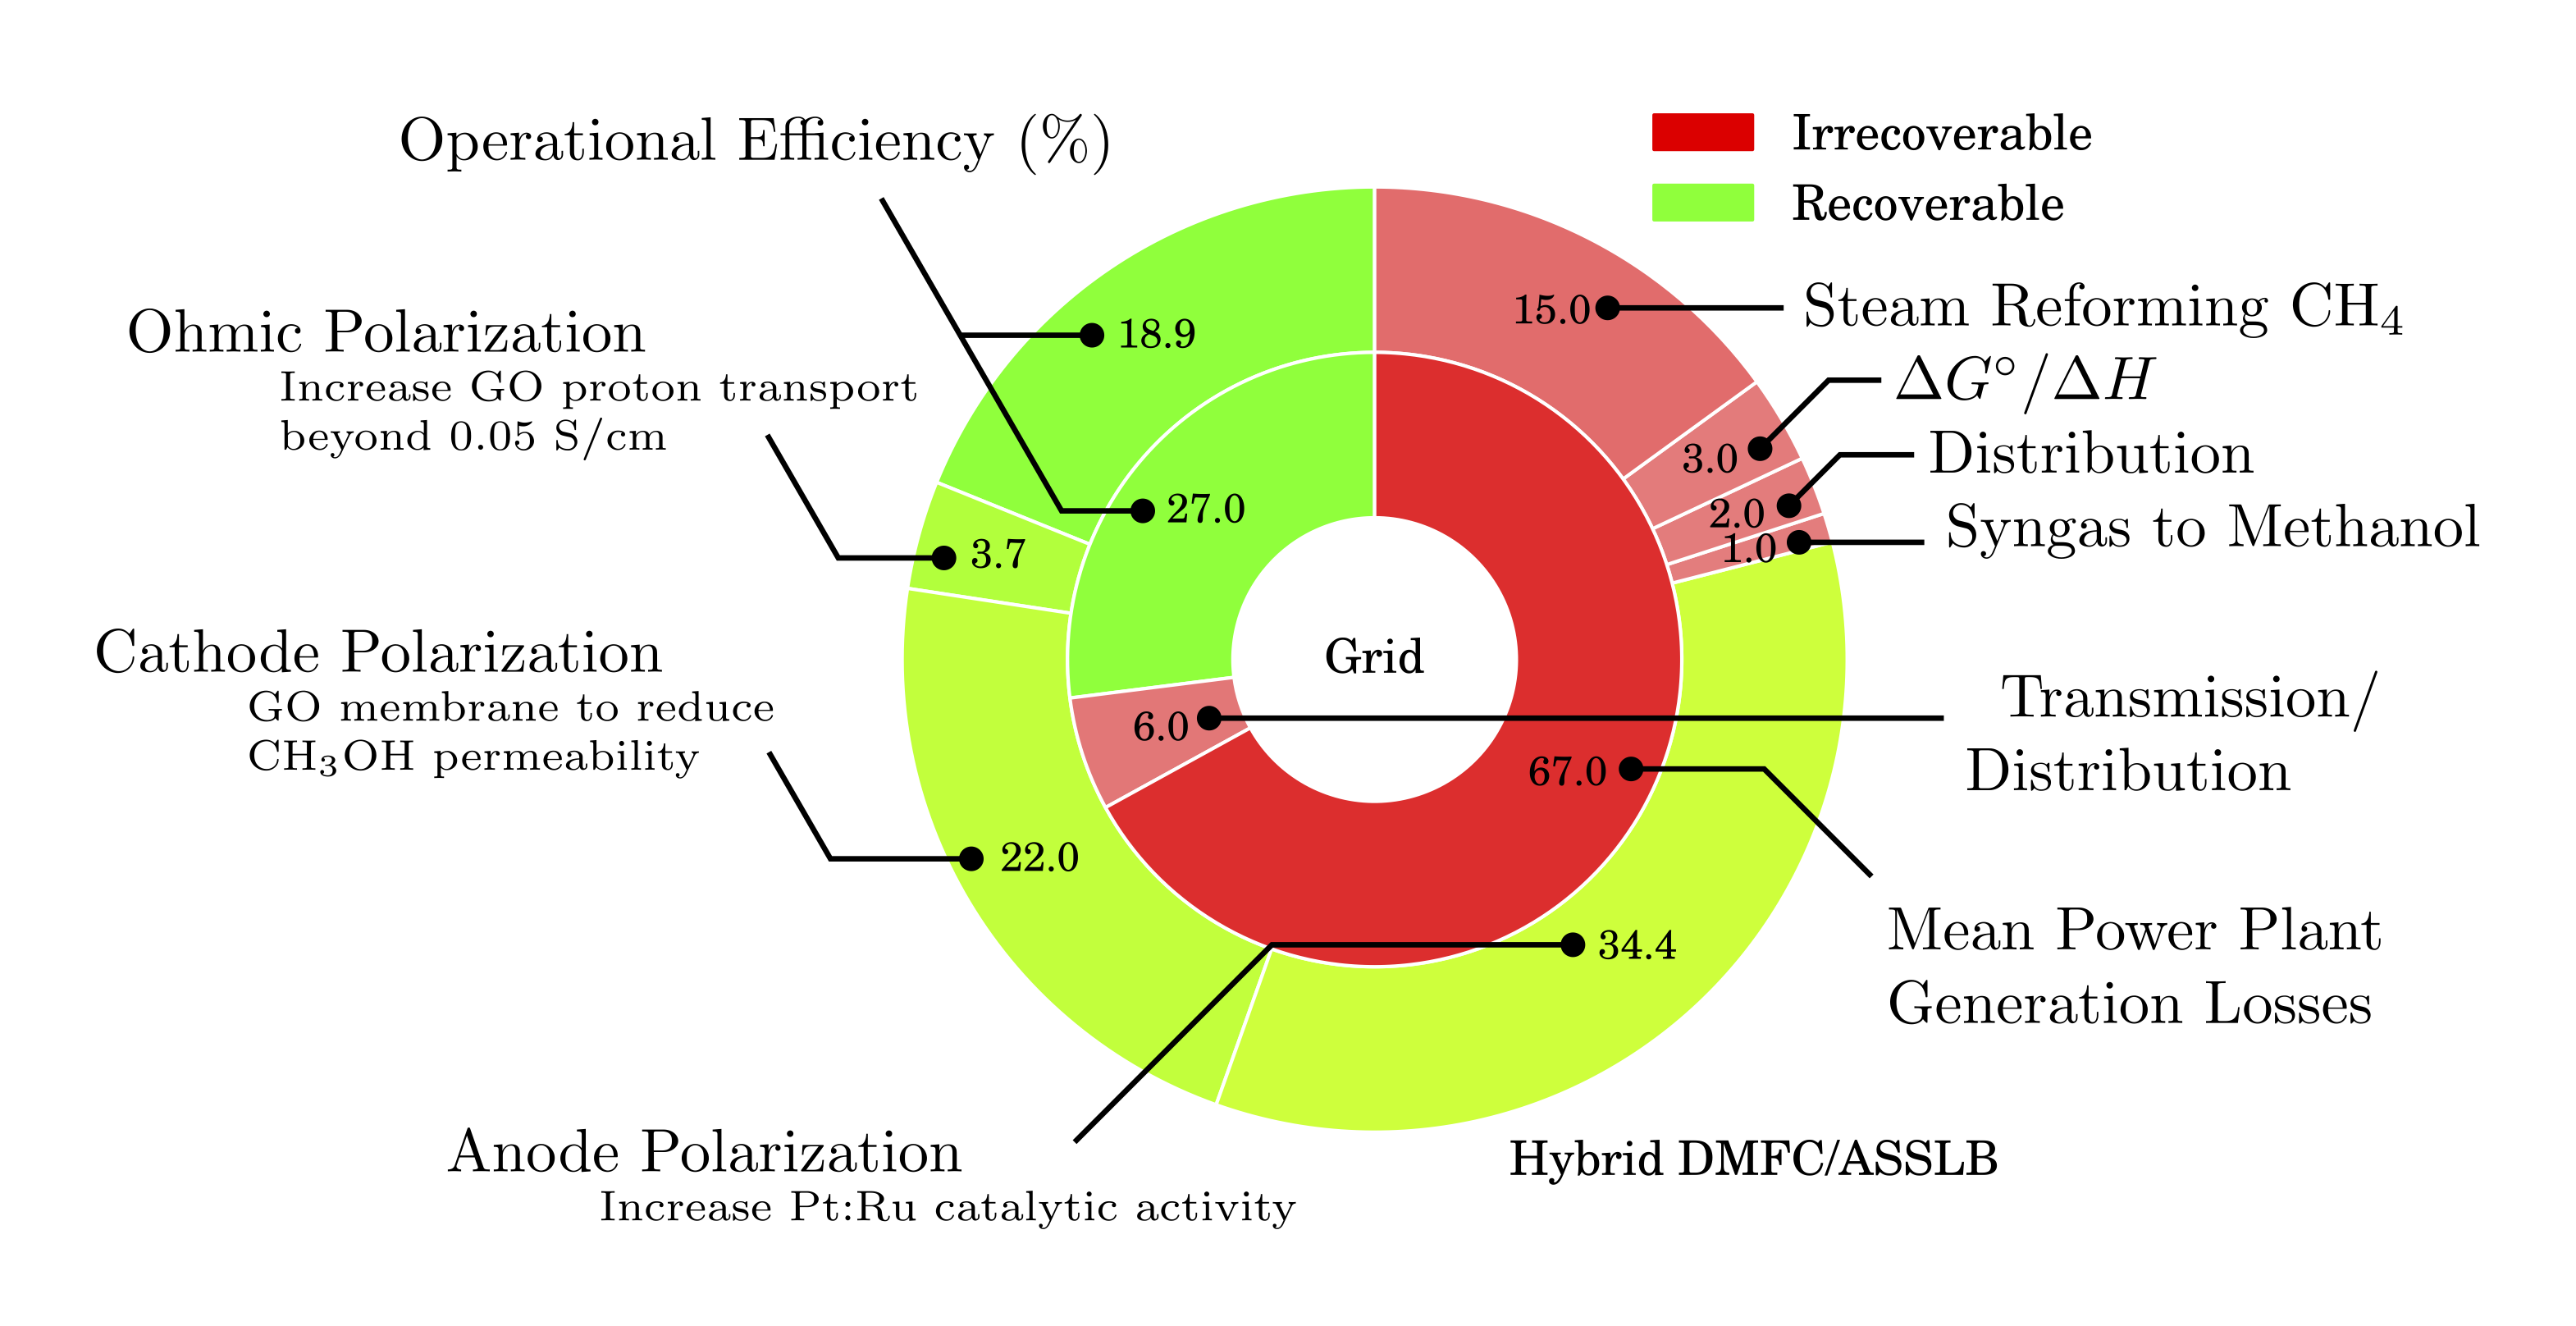
\includegraphics[width=0.48\textwidth]{fig/efficiency}
		\caption{Potential for improved energy efficiency through use of the proposed hybrid direct methanol fuel cell/all solid-state lithium battery power system.}
		\label{fig:efficiency}
	\end{center}
\end{wrapfigure}
This project will, over three years, address the three challenges facing DMFC that keep their efficiencies below our 35\% target efficiency: high methanol crossover, high anode polarization due to low catalyst activity, and high cathode polarization due to mixed potential losses. In order to reduce battery complexity, and improve the volumetric energy density of the hybrid power system, this project will improve battery technology through the development of an all solid-state lithium ion battery.  The resulting hybrid DMFC/ASSLB will allow the power and energy requirements of each application to be optimized independently.

\begin{minipage}{0.45 \textwidth}
	\begin{center}
	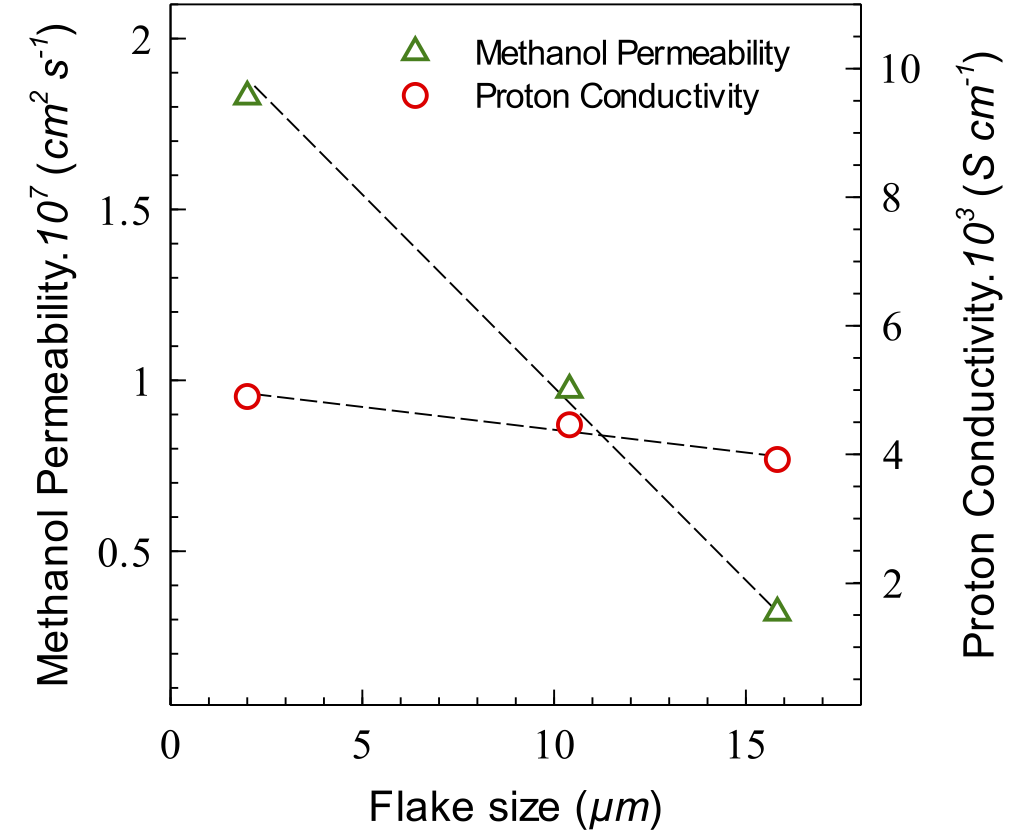
\includegraphics[width=\textwidth]{fig/Fig7Paneri2014}
	\captionof{figure}{Methanol permeability (diffusivity) and proton conductivity through graphene oxide (GO) as a function of the mean nanoplatelet size. From Paneri2014.}
	\label{fig:Fig7Paneri}
	\end{center}
\end{minipage} %
\hfill %
\begin{minipage}{0.45 \textwidth}
	\begin{center}
	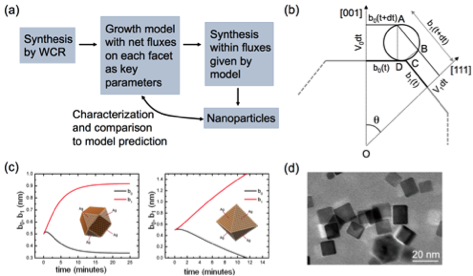
\includegraphics[width=\textwidth]{fig/NPModeling}
	\captionof{figure}{(a) Computationally guided synthesis of metallic nanoparticles by wet chemical reduction (WCR) �recent work at CSM (Leong2014) by Richards and Ciobanu. (b) Key parameters of the computational model: net attachment rates for each facet. (c) Predictions of the model for different ratios of attachement rates to (001) and (111) facets. (d) Actual Pd cuboctahedra synthesized by Richards' group.}
	\label{fig:NPModeling}
	\end{center}
\end{minipage} 
\vspace{1em}
\paragraph{\bf Proposed Work} Graphene oxide (GO) has recently been identified as a membrane with extremely high selectivity and permeability to water (Nair2012), but low intrinsic proton conductivity (Tateishi2013).  However, the proton conductivity of sulfonated GO has recently been shown to be comparable to that of Nafion${}^\textrm{\textregistered}$ (Sott2012a), but at the cost of increased methanol permeability (Jiang2014); furthermore, at high methanol concentrations the sulfonic acid groups on the GO surface induce a methanol/water phase separation that reduces proton conductivity (Paneri2014).  The precise nature of proton transport through GO is not known, but the insensitivity of proton transport to GO flake size (Figure~\ref{fig:Fig7Paneri}) suggests through-platelet transport plays a dominant role; contrarily, the decrease in methanol permeability over that same range indicates methanol permeation occurs predominantly at platelet edges.

Limited work has been done on the chemical modification of GO for DMFC membranes. The proposed work addresses two of the three problems: proton conductivity (ohmic losses) and methanol crossover (mixed potential losses).  We propose to modify the GO surface using vapor phase methods, including ALD and molecular layer deposition (MLD), to enable the development of GO membranes that resist methanol/water phase separation while increasing proton transport.  Molecular dynamics simulations of proton transport through graphene oxide will be used to evaluate the efficacy of chemically modified GO membranes.  For DMFC, success would be an increase in the metha-nol concentration from 2 to 10 M; a decrease in methanol permeability from 50 to 0.25~$\mathrm{mA/cm^2}$ (Zhao2009, Corti2014); and increase the proton conductivity for GO from 0.0045 to 0.05~S/cm (Paneri2014, Sone1996); and a twofold reduction in price, from \$550/kWh to \$250/kWh (Kamarudin2009).

Platinum group metal (PGM) catalyst activity is affected by both the nature of the substrate (Feng2013a) and by the shape and size of the catalyst nanoparticles (NPs).  The proposed effort will increase catalytic activity by optimization of the catalyst synthesis to produce nanoparticles of prescribed morphologies, shapes and sizes. We will pursue catalyst optimization by combining computational tools (synthesis models, simulations of process and properties) with synthesis and characterization to improve catalyst activity and achieve a fundamental understanding of their synthesis and/or control over the final product and its catalytic properties (Leong2014, example in Figure~\ref{fig:NPModeling}).

The catalytic materials systems to be addressed are metal and metal-alloy NPs, with or without core-shell morphologies.  These well-defined catalytic systems are ideal for linking experiments and modeling, providing controlled systems for building selective and complex functionalities.  The proposed effort will increase catalyst stability by lowering the solubility of Ru in acidic media. Our team has extensive experience in Pt-Ru deposition including wet chemical reduction (WCR), ALD, and sputtering.  In addition to technical challenges, catalyst cost poses a significant economic challenge.  Both anode and cathode require PGM catalysts.  Loading levels of 2.5 mg/cm2 account for a price of \$1366/kW (Pt: \$1162/oz).  To reduce catalytic loading, and bring the price below competing technologies, we will also investigate the targeted growth of Pt to GO surface defects using ALD, localizing catalyst deposition to the centers of proton transport.

Solid-state electrolytes appreciably reduce the complexity of each lithium ion cell, reducing both weight and volume.  With a smaller cell, this volume and weight can be recaptured into increased fuel storage, multiplying the impact of any improvement in battery performance.  An all solid-state battery using solid electrolytes is expected to have a higher energy density, reliability, and reduced safety concerns compared to a lithium ion battery using organic liquid electrolytes. All-solid-state batteries can be divided into two types, thin-film-type and bulk-type. For large-scale applications, bulk-type ASSLBs with high loadings of active material and solid electrolyte powders, are well suited because of their high energy density. However, ASSLBs have crucial challenges for practical applications, such as poor rate performance and poor contact be-tween the active material and the electrolyte.  Sulfide type electrolytes were developed to improve conductivity over earlier solid electrolytes, e.g. LiPON. $\mathrm{Li_2S}$--$\mathrm{P_2S_5}$ and $\mathrm{Li_2S}$--$\mathrm{P_2S_5}$--$\mathrm{GeS_2}$ systems offer ion conductivity from $10^{-3}$ to $10^{-2}$~S/cm at room temperature, similar to liquid electrolytes; and have a high, 5~V decomposition potential.  With these electrolytes, the maximum resistance is observed at the cathode/sulfide electrolyte interfaces. This presents the most pressing technical challenge: improved electrode -- specifically cathode -- contact with the electrolyte.

{\it Year 1} will focus on the development of individual components with significant progress toward the stated performance metrics.  This will include (1) synthesis and characterization of candidate graphene oxide and chemically modified GO membranes. (2) Synthesis, model-ing, and analysis of the stability, activity, and performance of the anode catalyst layer under conditions near and around those expected during fuel cell operation.  (3) We will use SEM, TEM, and cyclic voltammetry to understand the cathode/electrolyte interface, which has been identified as an issue of the greatest importance for the improvement in ASSLBs.  (4) Finally, system level modeling efforts will be put in place to pre-optimize operating conditions based on the evolving properties of the catalyst layer, membrane and battery properties.

{\it Year 2} will focus on attaining the target performance metrics for all individual components. Fuel cell components will be integrated into a test cell for controlled performance testing at the Energy Systems Integration Facility at NREL.  Solid-state battery components will be integrated into a coin cell configuration for electrochemical testing.

{\it Year 3} will optimize the performance of the integrated fuel cell and battery systems under simulated real-world operational variations. Merging the fuel cell and solid-state battery into a hybrid power system will be done at PGi.

Key technical risks for ALD and MLD modification of GO platelets reside in ineffective-ness of the sulfonic groups.  The risk will be mitigated our flexibility in pursuing alternative functionalizations and in our ability to model proton transport for a range of candidate functionalizations.  The Pt--Ru--R (R = N, C, B) catalysts may be susceptible to agglomeration, making their shape and chemistry ineffective.  Our team has explored additional functionalization of the carbon support with nitrogen to prevent aggregation in prior work and the capabilities are available to integrate this process to catalyst optimization.  The interplay between as-yet-unknown component properties under various operating conditions is a risk that will be mitigated through systems level modeling of fuel cell, battery, and hybrid system. By combining battery technology with direct methanol fuel cells, advancement in this hybrid system does not hinge on improvement in any single technology, but rather benefits from every individual improvement: in battery capacity, catalyst activity, or membrane performance.

\begin{center}\textbf{Team Organization and Capabilities}\end{center}

\noindent\textbf{Project Prime}: Process Global, Inc. (PGi) has established a unique partnership of highly experienced industry leaders representing a multidisciplinary range of disruptive technologies. The core team has over 100+ man-years of experience across a wide range of fields, including manufacturing, process development, equipment engineering, and renewable energy.

\noindent\textit{Principle Investigator}: Dr. Branden Kappes is the VP of Technology at PGi.  He will be responsible for systematically studying electrochemical properties of the solid-state Li-ion battery and characterization and testing of the proposed hybrid power system.

\noindent\textbf{Project Partner}: NREL has a strong research effort in fuel cell catalyst development which includes:  metal alloy WCR, ALD, sputtering; physical and chemical modification of fuel cell catalyst support; synthesis of advanced carbon materials; electrochemical testing and cycling; physical characterization of materials; fuel cell assembly and testing. NREL is also equipped with an electrochemical laboratory that houses several multichannel potentiostat-galvanostats for data acquisition and computerized electronic control of voltages and currents delivered to electrochemical test cells, and electrochemical analysis station for characterizing and analysis of electrochemical properties. There are capabilities for full coin cell fabrication, including Argon-filled glove-box, a film applicator, compressor and crimper to conduct cycling at elevated temperatures.

\noindent\textit{Key Member}: Dr. Chunmei Ban is staff scientist of the Center of Chemistry and Materials Sci-ence at the National Renewable Energy Laboratory (NREL). Dr. Ban�s expertise in the study of nanostructured materials has been instrumental in successfully implementing DOE-funded projects including Nanostructured Metal Oxide and high-energy electrode materials for lithium-ion batteries.

\noindent\textit{Key Member}: Dr. Steven Christensen is an expert in catalyst characterization and will support process feedback for the optimization of the DMFC components.

\noindent\textit{Key Member}: Dr. Katherine Hurst is an expert in material synthesis and will perform catalyst synthesis and GO formation and modification.

\noindent\textbf{Project Partner}: Colorado School of Mines maintains a strong institutional focus on energy re-search, including high performance computing resources dedicated to solving energy-related challenges using modeling and simulation, and extensive research in fuel cells through the Colorado Fuel Cell Center.

\noindent\textit{Key Member}: Prof. Cristian Ciobanu is an expert in computational materials science focusing on structure, properties, and phenomena in nanomaterials, and will provide molecular dynamics simulations and process modeling expertise to the project.

Within the last three years, all members of the current team have collaborated on projects rele-vant to the proposed effort. Drs. Ban and Kappes collaborated on organic flow batteries through the ARPA-E sponsored RANGE program, have collaborated for three years on the design and synthesis of nanostructured materials for next-generation Li-ion batteries, and are coauthors on several publications on materials for lithium ion batteries. Drs. Ciobanu and Kappes have collab-orated extensively on simulation and modeling across a range of materials challenges, including research into lithium ion batteries.

\end{document}  